\section{Agentic Simulation: Data Synthesis, User Simulation, and Environment Simulation}
\label{sec:simulation}

In this survey, \emph{simulation} refers to using one or more agents to approximate parts of the recommendation ecosystem that are expensive, unsafe, or impossible to observe directly.
This includes generating synthetic training data, simulating user feedback to train or test recommenders, and simulating closed-loop environments where recommender policies interact with populations over time. 




\subsection{Why do we need simulation?}\label{subsuc:simulation_motivation}
Across the literature, simulation is used for four recurring motivations: 
1) \textbf{Training without expensive interaction.} Simulators provide behavioral signals when online exploration is infeasible (cold-start, privacy constraints, or limited traffic). 
2) \textbf{Counterfactual and stress testing.} Simulators enable controlled tests of robustness, fairness, and safety properties that are difficult to measure from logs. 
3) \textbf{Data synthesis and augmentation.} Synthetic dialogues, profiles, and feedback can reduce sparsity and broaden coverage. 
4) \textbf{Ecosystem and feedback-loop analysis.} Multi-agent simulations can model long-term dynamics such as filter bubbles and echo chambers. 


\subsection{A taxonomy of simulation types}
We propose a simple taxonomy that aligns with autonomy and the “what is being simulated” question.

\begin{figure}[t]
\setlength{\abovecaptionskip}{-0.0cm}  % caption与图之间（默认10pt）
\setlength{\belowcaptionskip}{-0.0cm} % caption与下方正文之间
    \centering
    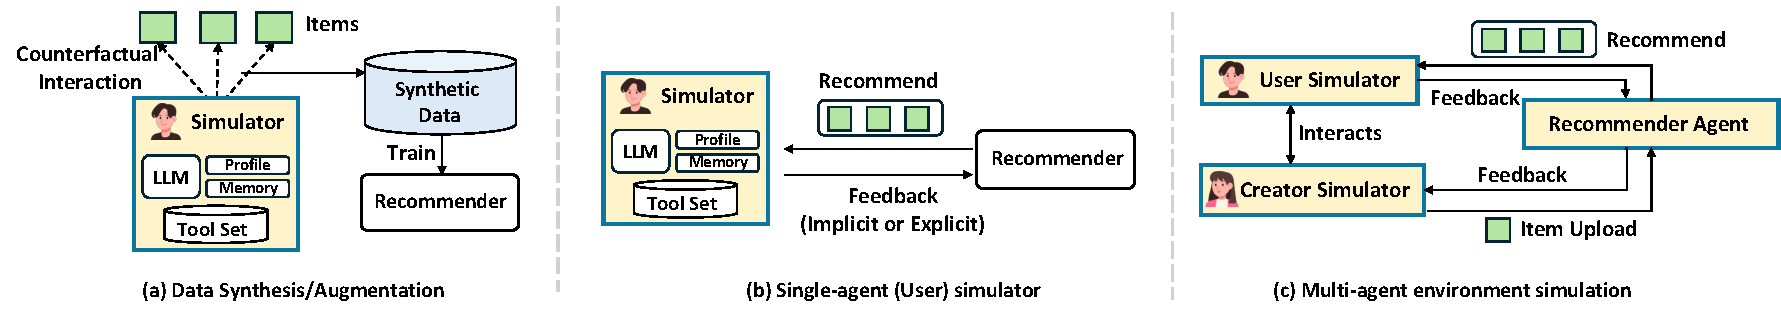
\includegraphics[width=1\linewidth]{figures/simulation.pdf}
    \caption{Three taxonomies of agentic simulation: data synthesis, user (single-agent) simulation, and environment (multi-agent) simulation.}
    \label{fig:simulation}
\end{figure}

\subsubsection{\textbf{(1) Data synthesis / data augmentation}}\label{subsubsec:simulation-data-synthesis}
Data synthesis uses agents to generate artifacts that support training or evaluation: synthetic conversations, item descriptions, preference rationales, or structured user profiles.
TalkPlayData~2 exemplifies an agentic synthetic pipeline for multi-modal conversational music recommendation, demonstrating how agentic generation can create richer training signals than template-based augmentation \cite{choi2025talkplaydata}. 
For cold-start settings, simulator-style generation can replace missing interaction histories with plausible synthetic signals: a large language model simulator for cold-start recommendation explicitly targets the absence of real user interaction data \cite{huang2025large}.  
LAUS~\cite{park2025llm} leverages large language models to simulate user interactions, enabling the training of news recommenders without relying on large-scale real user data.
For reinforcement learning-based recommender systems, \citet{zhang2025llm} propose an interpretable user simulator that combines LLM-based preference reasoning with statistical behavior modeling to generate high-fidelity training data, thereby improving recommendation training.






\subsubsection{\textbf{(2) User simulation (single-agent simulators)}}\label{subsubsec:simulation-single-agent-simulator}
User simulation models user feedback (clicks, ratings, critiques, dialogue acts) conditioned on context.
This can appear as a single LLM agent that plays the user role, or as structured simulators augmented by LLM reasoning. 
A key example is RecAgent, which frames simulation as a paradigm for recommender systems and highlights how LLM agents can generate interactive trajectories rather than static labels \cite{wang2023recagent}.
User Behavior Simulation with LLM-based Agents provides a systematic formulation and is especially relevant because it positions LLM-agent simulators as a way to reproduce behavioral dynamics at scale \cite{wang2025user}, requiring alignment with real-world data distributions. 


\paragraph{\textbf{Design axes for user simulators.}}
User simulators can be compared along:
(i) \textbf{fidelity} (does the simulator match real distributions and causal responses?),
(ii) \textbf{controllability} (can we steer demographics, noise, and drift?),
(iii) \textbf{observability} (does the simulator output only implicit feedback or also explicit rationales?),
and (iv) \textbf{calibration} (does the simulator’s actions reflect real behaviors?).
These axes should be evaluated explicitly rather than assumed, because simulator errors can lead to “training on simulator artifacts.” 
In the following, we discuss the existing literature from these design axes, respectively. 


(i) \emph{Simulation fidelity}. To ensure high simulation \emph{fidelity} aligned with real-world data distributions, user simulators primarily focus on two aspects: {\textit{profile construction}} and {\textit{memory design}}.
\begin{itemize}
    \item \textbf{\textit{Profile construction}}. Most existing user simulators construct personalized user profiles from real-world interaction data~\cite{wanyan2025temporal,liu2025diagnostic}. For example, RecAgent~\cite{recagent} and Lusifer~\cite{ebrat2025lusifer} build basic profiles using demographic and attribute information such as gender, age, traits, and interests, while Agent4Rec~\cite{zhang2024agent4rec} derives social traits (e.g., activity, conformity, and diversity) from datasets like MovieLens-1M. In addition, several methods, including RecAgent~\cite{wang2023recagent} and Agent4Rec~\cite{zhang2024agent4rec}, leverage LLMs for generative profiling, such as summarizing representative behavioral roles, personalized preferences, and rating patterns.
    \item \textbf{\textit{Memory design}}. Another key component to ensure fidelity is memory. It allows the agent to recall past actions, feedback, and outcomes, thereby supporting sequential decision-making and adaptive behavior in long-term recommendation simulations. 
    Beyond saving long- and short-term interests, memory mechanisms in user simulators are designed to capture richer aspects of user behavior. For instance, RecAgent~\cite{recagent} introduces sensory memory, which directly interacts with the environment and transforms raw observations into concise representations. Agent4Rec~\cite{zhang2024agent4rec} proposes factual memory, which encodes user interaction behaviors, and emotional memory, which captures the psychological states induced by these interactions.
\end{itemize}


(ii) \emph{Simulator controllability}. A controllable user simulator adds an important dimension: \emph{controllability} over behavior and dynamics, which is critical for evaluation and for testing robustness to demographic or preference shifts \cite{zhu2025llm,wei2025mirroring,zhu2024reliable}. 
\citet{zhu2025llm} proposes a plugin-based, controllable and human-in-the-loop LLM user simulator (CSHI), where controllability is enabled by a modular plugin manager for stage-wise behavior control, explicit user profile manipulation, and human intervention.
Additionally, controllability can be achieved by adjusting the simulator’s memory decay rate to model interest drift~\cite{wang2023recagent, ye2025creagent}, and by tuning the sampling distribution of user profiles to simulate different demographic compositions~\cite{ye2025creagent, zhang2024agent4rec}. 



(iii) \emph{Simulation observability}. Beyond outputting implicit feedback (e.g., like), improving \emph{observability} of the recommendation process is another key ability of user simulator. \citet{zhang2025llm} propose an interpretable user simulator that integrates LLM-based preference reasoning with statistical behavior modeling to generate high-fidelity training data, thereby improving reinforcement learning–based recommender systems.
For domain-specific simulators, LLM-as-user simulation for news recommendation targets training without real interactions \cite{park2025llm}, while Lusifer provides an LLM-based simulated feedback environment for online recommender systems \cite{ebrat2025lusifer}.

(iv) \textit{Behavior calibration}. 
Whether the simulator’s behavior reflects real user behavior is a critical aspect of simulator design. Existing research primarily models two types of actions: (1) user-system actions and (2) user-user actions.

\begin{itemize}
    \item 
\textbf{User-system action.} In non-conversational user simulation, implicit signals (e.g., like, click)~\cite{zhang2024agent4rec, park2025llm, zhang2025llm, huang2025large, bougie2026alignuser} and explicit signals (e.g., comments, reviews)~\cite{recagent} constitute the two primary types of user-to-item actions in user simulation. To implicitly model,
Agent4Rec~\cite{zhang2024agent4rec} divides user page-by-page browsing actions into taste-driven and emotion-driven types: (1) taste-driven actions include viewing, rating, and expressing post-viewing feelings towards items, capturing users’ immediate preferences during page-by-page recommendations; (2) emotion-driven actions (i.e. existing the session or rating the recommender system) capture user affective states and reflect how satisfaction and fatigue shape their decision to continue or quit. Beyond user feedback simulation, some works~\cite{ye2025creagent, jin2025recinter} model item providers (e.g., creators or merchants), enabling simulators to update item attributes or generate new items to capture supply-side dynamics.
In conversational recommender systems, users typically interact with the system through the generative capabilities of LLMs~\cite{chen2025recusersim, feng2025expectation}, generating fluent and contextually relevant responses to express preference.




\item \textbf{User-user action.} 
To capture this broader social dimension, recent works~\cite{recagent} introduce conversational user simulators that equip LLM-based agents with the ability to interact with other user simulators, enabling more realistic and socially grounded simulations.
RecAgent~\cite{recagent} not only enables users to perform conventional recommender system actions (e.g., searching, browsing), but also allows agents to engage in one-to-one chatting and one-to-many broadcasting. 



    
\end{itemize}
% 



\subsubsection{\textbf{(3) Closed-loop multi-agent environment simulation}}\label{subsubsec:simulation-closed-loop-multi-agent-environment}
The most ambitious form of simulation uses multiple agents to model populations and platform mechanisms, enabling closed-loop experiments over long horizons.
RecoWorld provides simulated environments for agentic recommender systems, pushing toward standardized testbeds where policies can be compared under controlled dynamics \cite{liu2025recoworld}.
Filter bubble simulation with LLM agents demonstrates that such environments can capture emergent societal effects (e.g., self-reinforcing exposure patterns) that are central to multi-objective evaluation \cite{sukiennik2025simulating}. 
GGBond extends this direction with a graph-based AI-agent society, highlighting the need to represent social structure and influence in ecosystem simulations \cite{zhong2025ggbond}. 
\citet{cai2025agentic} proposes an agentic feedback loop framework that explicitly models the iterative interaction between a recommendation agent and a user agent, allowing both to co-evolve and improve through mutual feedback.
Beyond user simulation, recent works extend the paradigm to multi-agent environments by modeling item providers  (e.g., merchants, content creators). In this setting, simulators can act not only as a user model that mimics user behavior passively responding to recommendations, but also as an active recommendation agent that proactively generates and recommends items to other users. For example, CreAgent~\cite{ye2025creagent} leverages LLMs to simulate a realistic content recommendation platform (i.e., YouTube) involving both users and content creators, enabling long-term offline evaluation of recommender systems with multi-stakeholders. RecInter~\cite{jin2025recinter} introduces merchant agents that can respond to user feedback and dynamically modify item attributes, enabling a more realistic co-evolution of users, items, and providers. 




\subsection{Simulation shortcoming and open challenges}
Despite rapid progress, simulation brings substantial risks: 
1) \textbf{Simulator--policy mismatch.}
Agents trained against a simulator may overfit to simulator quirks, leading to inflated offline performance and poor real-world transfer. This is particularly problematic for agentic systems that exploit loopholes in feedback generation. 
2) \textbf{Compounding error in closed loops.}
In closed-loop simulation, small misspecifications in user response can compound over time, producing misleading conclusions about long-term welfare. 
3) \textbf{Evaluation of simulators themselves.}
Simulators must be evaluated as \emph{models}, not just used as tools. We argue that simulator evaluation should be treated as a first-class part of agentic recommender evaluation (Sec.~\ref{sec:evaluation}), including calibration tests, distributional similarity tests, and targeted behavioral probes. 
4) \textbf{Link to evaluation.}
Simulation is simultaneously an \emph{object} of evaluation and a \emph{method} for evaluation; for agentic recommendation, the two are inseparable. We therefore treat simulation-based evaluation and red-teaming as core methodologies in the next section.








